% Format teze zasnovan je na paketu memoir
% http://tug.ctan.org/macros/latex/contrib/memoir/memman.pdf ili
% http://texdoc.net/texmf-dist/doc/latex/memoir/memman.pdf
% 
% Prilikom zadavanja klase memoir, navedenim opcijama se podešava 
% veličina slova (12pt) i jednostrano štampanje (oneside).
% Ove parametre možete menjati samo ako pravite nezvanične verzije
% mastera za privatnu upotrebu (na primer, u b5 varijanti ima smisla 
% smanjiti 
\documentclass[12pt,oneside]{memoir} 

% da bi se u sadrzaju video subsection
\setcounter{tocdepth}{3}
\setsecnumdepth{subsubsection}

% definicije
\newtheorem{definition}{Definicija}

%find i copy/paste
\usepackage{cmap}

\usepackage{caption}
\usepackage{subcaption}

% razmak medju paragrafima
\setlength{\parskip}{1em}

% linkovi u sadržaju
\usepackage{hyperref}
\hypersetup{
    colorlinks,
    citecolor=blue,
    filecolor=black,
    linkcolor=blue,
    urlcolor=black
}

% Paket koji definiše sve specifičnosti master rada Matematičkog fakulteta
\usepackage[latinica]{matfmaster} 

%bibliografija
\bib{rad}


%
% Podrazumevano pismo je ćirilica.
%   Ako koristite pdflatex, a ne xetex, sav latinički tekst na srpskom jeziku
%   treba biti okružen sa \lat{...} ili \begin{latinica}...\end{latinica}.
%
% Opicija [latinica]:
%   ako želite da pišete latiniciom, dodajte opciju "latinica" tj.
%   prethodni paket uključite pomoću: \usepackage[latinica]{matfmaster}.
%   Ako koristite pdflatex, a ne xetex, sav ćirilički tekst treba biti
%   okružen sa \cir{...} ili \begin{cirilica}...\end{cirilica}.
%
% Opcija [biblatex]:
%   ako želite da koristite reference na više jezika i umesto paketa
%   bibtex da koristite BibLaTeX/Biber, dodajte opciju "biblatex" tj.
%   prethodni paket uključite pomoću: \usepackage[biblatex]{matfmaster}
%
% Opcija [b5paper]:
%   ako želite da napravite verziju teze u manjem (b5) formatu, navedite
%   opciju "b5paper", tj. prethodni paket uključite pomoću: 
%   \usepackage[b5paper]{matfmaster}. Tada ima smisla razmisliti o promeni
%   veličine slova (izmenom opcije 12pt na 11pt u \documentclass{memoir}).
%
% Naravno, opcije je moguće kombinovati.
% Npr. \usepackage[b5paper,biblatex]{matfmaster}

% Pomoćni paket koji generiše nasumičan tekst u kojem se javljaju sva slova
% azbuke (nema potrebe koristiti ovo u pravim disertacijama)
\usepackage[latinica]{}%{pangrami}

% Datoteka sa literaturom u BibTex tj. BibLaTeX/Biber formatu
%\bib{matfmaster-primer}

% Ime kandidata na srpskom jeziku (u odabranom pismu)
\autor{Nikola Z. Vidič}
% Naslov teze na srpskom jeziku (u odabranom pismu)
\naslov{Primena mašinskog učenja u verifikaciji softvera}
% Godina u kojoj je teza predana komisiji
\godina{2018}
% Ime i afilijacija mentora (u odabranom pismu)
\mentor{dr Milena \textsc{Vujošević Janičić}, docent\\ Univerzitet u Beogradu, Matematički fakultet}
% Ime i afilijacija prvog člana komisije (u odabranom pismu)
\komisijaA{dr Mladen \textsc{Nikolić}, docent\\ Univerzitet u Beogradu, Matematički fakultet}
% Ime i afilijacija drugog člana komisije (u odabranom pismu)
\komisijaB{dr Filip \textsc{Marić}, vanredni profesor\\ Univerzitet u Beogradu, Matematički fakultet}
% Ime i afilijacija trećeg člana komisije (opciono)
% \komisijaC{}
% Ime i afilijacija četvrtog člana komisije (opciono)
% \komisijaD{}
% Datum odbrane (odkomentarisati narednu liniju i upisati datum odbrane ako je poznat)
% \datumodbrane{}

% Apstrakt na srpskom jeziku (u odabranom pismu)

\apstr{%
%\pangrami
}

% Ključne reči na srpskom jeziku (u odabranom pismu)
\kljucnereci{}%analiza, geometrija, algebra, logika, računarstvo, astronomija}

\begin{document}
% ==============================================================================
% Uvodni deo teze
\frontmatter
% ==============================================================================
% Naslovna strana
\naslovna
% Strana sa podacima o mentoru i članovima komisije
\komisija
% Strana sa posvetom (u odabranom pismu)
\posveta{}%Mami, tati i dedi}
% Strana sa podacima o disertaciji na srpskom jeziku
\apstrakt
% Sadržaj teze
\tableofcontents*

% ==============================================================================
% Glavni deo teze
\mainmatter
% ==============================================================================

% ------------------------------------------------------------------------------
\chapter{Uvod}
% ------------------------------------------------------------------------------
%\pangrami




\chapter{Mašinsko učenje}
\label{chp:mašinsko učenje}

%Termin \textit{mašinsko učenje (eng. machine learning)} nastaje 1959-te godine, a njegov tvorac je Artur Semjuel (Arthur Samuel) američki pionir u poljima kompjuterskih igara i \textit{veštačke inteligencije (eng. artificial intelligence)}. 
%Sama ideja mašinskog učenja javlja se još ranije, u radovima Alena Tjuringa (Alan Turing) četrdesetih godina dvadesetog veka. %Mašinsko učenje nastaje iz potrage za veštačkom inteligencijom. 
%Razvoj mašinskog učenja vođen je željom da se razume i oponaša ljudski potencijal za učenje. 
%Ubrzo nakon što veštačka inteligencija postaje univerzitetska disciplina pojavljuju se naučnici zainteresovani da vide kako mašine uče na osnovu podataka. Prvi pokušaji takvog načina učenja bili su u vidu \textit{neuronskih mreža (eng. neural networks)} koje su pedesetih godina najčešće imale formu \textit{perceptrona (eng. perceptron)}. 

Sama ideja \textit{mašinskog učenja (eng. machine learning)} javlja se još četrdesetih godina dvadesetog veka u radovima Alana Tjuringa (Alan Turing). Razvoj mašinskog učenja vođen je željom da se razume i oponaša ljudski potencijal za učenje. Pedesetih godina mašinsko učenje se razvija zajedno sa pojmom perceptrona, pretka neuronskih mreža. Razvoj mašinskog učenja u formi neuronskih mreža nastavlja se sve do devedesetih godina. Početkom dvehiljaditih dešava se proboj na polju razvoja \textit{veštačke inteligencije (eng. artificial inteligence)} i mnogi problemi za koje se smatralo da će jos dugo ostati nerešeni bivaju rešeni, velikim delom zahvaljujući mašinskom učenju. Uopšteno, ,,mašinsko učenje predstavlja disciplinu koja se bavi konstrukcijom sistema koji se prilagođavaju i popravljaju svoje performanse sa povećanjem iskustva, oličenog u količini relevantnih podataka''[mladen]. Mašinsko učenje proučava indukcijski način zaključivanja tj. generalizaciju (uopštavanje ka univerzalnim zaključcima). Primene mašinskog učenja su brojne: prepoznavanje lica na slikama, oblika na slikama, prepoznavanje tumora, autonomno upravljanje automobilima, autonomno letenje, igranje igara na tabli kao što je šah, klasifikacija teksta, prepoznavanje cifara i mnoge druge \cite{mladen}.

Mašinsko učenje za rešavanje problema koristi različite metode. Ove metode se prema prirodi problema učenja svrstavaju u jednu od tri grupe: \textit{nadgledano učenje} (eng. \textit{supervised learning}), \textit{nenadgledano učenje} (eng. \textit{unsupervised learning}) ili \textit{učenje potkrepljivanjem} (eng. \textit{reinforcement learning}). 
Nadgledano učenje se odlikuje ulaznim podacima tj. podacima na osnovu kojih se uči i izlaznim podacima tj. podacima koje je potrebno naučiti. Naziv je posledica sličnosti postupka nadgledanog učenja i učenja u kome profesor zada učeniku zadatke i nakon što ih učenik reši, da učeniku odgovore radi poređenja rezultata. Algoritmi mašinskog učenja se opisuju kao učenje ciljne funkcije \textit{f} koja najbolje opisuje vezu između ulaznih promenljivih \textit{x} i izlazne promenljive \textit{y}, odnosno $y=f(x)$. Naučena veza (ciljna funkcija $f$) se kasnije koristi za buduća predviđanja izlaza $y$ na osnovu novih vrednosti ulaza $x$. Najčešće je ulaz predstavljen vektorom vrednosti promenljivih koje se nazivaju \textit{atributima} (eng. \textit{features}), a izlaz kao jedna promenljiva koja se zove \textit{ciljna promenljiva} (eng. \textit{target variable}). 
Kako se u današnje vreme raspolaže ogromnim količinama podataka merenim gigabajtima i terabajtima, neophodno je pronaći metode koje automatski pronalaze veze između promenljivih. Veze tj. izgrađene ciljne funkcije se nazivaju \textit{modelima mašinskog učenja}. Postoji veliki broj modela i ne opisuju svi podjednako dobro veze među podacima. Od kvalitetnog modela se očekuje da vrši dobru generalizaciju tj. da prilikom predviđanja retko greši \cite{mladen, mlm-how-alghoritms-work}. %https://machinelearningmastery.com/how-machine-learning-algorithms-work/

Osnovne vrste nadgledanog učenja su \textit{klasifikacija} i \textit{regresija} \cite{mladen}.
\begin{itemize}
\item ,,Klasifikacija je problem predviđanja kategoričke ciljne promenljive.'' Vrednosti kategoričke promenljive pripadaju nekom konačnom skupu, pri čemu ne postoji uređenje među tim vrednostima. 
\item ,,Regresija je problem predviđanja neprekidne ciljne promenljive''.  Neprekidne promenljive uzimaju vrednosti iz neograničenog skupa vrednosti.
 \end{itemize}

U nastavku će detaljnije biti opisani modeli klasifikacije zasnovani na algoritmima \textit{k} najbližih suseda, 
slučajnim šumama i logističkoj regresiji.

%% kNN
\section{Algoritam \textit{k} najbližih suseda}

Klasifikatori zasnovani na algoritmu \textit{k} najbližih suseda spadaju u klasifikatore zasnovane na instancama. Klasifikatori zasnovani na instancama spadaju u neparametarske modele. Takvi modeli ne mogu se opisati konačnim skupom parametara i oni moraju da čuvaju skup podataka za trening na osnovu koga se vrši klasifikacija novih instanci. Dakle, kod modela zasnovanih na instancama ne postoji eksplicitan model već je model sadržan u skupu trening instanci. Sva izračunavanja vrše se u fazi predviđanja. Ovi klasifikatori svoju predikciju zasnivaju na lokalnim podacima pa su stoga podložni greškama zbog postojanja šuma. Zavisni su od izbora mere bliskosti i adekvatnog preprocesiranja podataka. Ako vrednosti atributa imaju skale različitih vrednosti, jedan atribut može više uticati na ishod klasifikacije a da to nije opravdano. Ovo se može rešiti svođenjem atributa na istu skalu standardizacijom. Pored svoje jednostavnosti, ovi modeli nalaze široku primenu \cite{mladen, mitic}.\par

Objekti podaci koje koristi metod najbližih suseda najčešće su predstavljeni kao tačke u \textit{d}-dimenzionom prostoru, gde je \textit{d} broj atributa objekata. Pretpostavlja se da postoji rastojanje među objektima kao i metrika koja definiše to rastojanje. Ideja vodilja primene metoda najbližih suseda je izreka : ,,Ako hoda kao patka, priča kao patka i izgleda kao patka, onda je najverovatnije patka'' \cite{mladen, mitic}. \par

\subsection{Dodeljivanje klase objektu}
%\textbf{Dodeljivanje klase objektu} 
Prilikom klasifikacije nepoznatog objekta prvo se među poznatim objektima pronađe njegovih \textit{k} najbližih suseda na osnovu izabrane mere bliskosti (često je u upotrebi \textit{Euklidsko rastojanje}).% Najbliži susedi objekta odgovaraju najbližim tačkama u prostoru. 
Algoritam novom objektu pridružuje klasu koja se \textit{najčešće javlja među njegovim susedima} (eng. \textit{majority voting}). U slučaju nerešenog ishoda, klasa nepoznatog objekta se dobija slučajnim izborom iz skupa najzastupljenijih klasa. Da bi se izbegli nerešeni ishodi, česta je praksa da se za \textit{k} uzima neparan broj \cite{mitic, mladen}.%eosl] 
\par

\begin{figure}[!ht]
    \centering
    \begin{subfigure}[b]{0.3\textwidth}
        \centering
        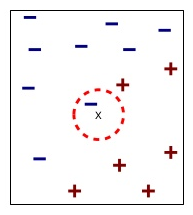
\includegraphics[width=\textwidth]{knna}
        \caption{\textit{k}=1}
        \label{fig:knna}
    \end{subfigure}
    \hfill
    \begin{subfigure}[b]{0.3\textwidth}
        \centering
        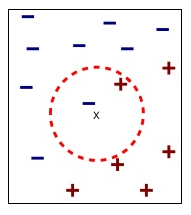
\includegraphics[width=\textwidth]{knnb}
        \caption{\textit{k}=2}
        \label{fig:knnb}
    \end{subfigure}
    \hfill
    \begin{subfigure}[b]{0.3\textwidth}
        \centering
        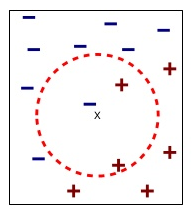
\includegraphics[width=\textwidth]{knnc}
        \caption{\textit{k}=3}
        \label{fig:knnc}
    \end{subfigure}
    \caption{Susedstva i dodeljivanje klasa novoj instanci za \textit{k}=1, 2 i 3}
    \label{fig:knn}
\end{figure}

Na slici \ref{fig:knn} prikazana su susedstva instance koja se nalazi u sredini kruga kada algoritam \textit{k} najbližih suseda uzima vrednosti 1, 2 i 3 za \textit{k}. Instanci će biti dodeljena klasa na osnovu klasa njenih najbližih suseda. Na slici \ref{fig:knna} klasa najbližeg suseda je (-) pa će i klasa instance biti (-). U slučaju \ref{fig:knnc} dva suseda su klase (+), a jedan klase (-) pa će klasa instance biti (+). Slika \ref{fig:knnb} ilustruje situaciju podjednake zastupljenosti klasa (jedan (+) i jedan (-)). U ovakvim situacijama, instanci se dodeljuje klasa slučajnim izborom. \cite{mitic}

Za rezultat klasifikacije jako je bitan izbor parametra \textit{k}. U slučaju male vrednosti parametra \textit{k} može doći do preprilagođavanja. Do grešaka dolazi jer je mali broj suseda uključen u razmatranje. Često se može javiti greška zbog prisustva šuma. Sa druge strane, velika vrednost parametra \textit{k} vodi ka potprilagođavanju. U tom slučaju do greške može doći jer se razmatraju klase onih objekata koji nisu u neposrednom susedstvu \cite{mladen, mitic}.

%% LR
\section{Logistička regresija}

Logistička regresija predstavlja probabilistički model klasifikacije. Koristi se i za probleme binarne i višeklasne klasifikacije. Kod probabilističkih modela je potrebno definisati raspodelu verovatnoće koju kasnije treba oceniti na osnovu podataka. Da bi ocena raspodele bila računski izvodljiva potrebno je uvesti pretpostavke o raspodeli podataka i međusobnoj zavisnosti promenljivih. Pogrešne pretpostavke o podacima, njihovoj raspodeli i zavisnosti, vode ka lošijim rezultatima predviđanja. U daljem tekstu detaljnije je opisana binarna logistička regresija \cite{mladen}.

Logistička regresija pretpostavlja međusobnu nezavisnost vrednosti ciljne promenljive  \textit{y} i  \textit{Bernulijevu raspodelu} ciljne promenljive  \textit{y} za date vrednosti atributa  \textit{x}. To znači da postoji parametar  $\mu$ iz intervala [0,1] takav da je  \textit{p}(\textit{y}=1|\textit{x}) = $\mu$, a  \textit{p}(\textit{y}=0|\textit{x}) = 1-$\mu$. Ovako definisan model logističke regresije nije kompletan. Potrebno je definisati zavisnost parametra $\mu$ od vrednosti atributa \textit{x}. Da bi se parametar $\mu$ uklopio u definiciju verovatnoće, njegove vrednosti moraju biti u intervalu [0,1]. Poželjno bi bilo koristiti model linearne regresije zbog njegove jednostavnosti i lake interpretabilnosti, ali na prvi pogled ovo nije moguće jer vrednosti linearnog modela pripadaju intervalu [$-\infty$, $\infty$]. Međutim, moguće je koristiti model linearne regresije ako se njegove vrednosti transformišu nekom nenegativnom, monotonom, neprekidnom i diferencijabilnom funkcijom u interval [0,1]. U tu svrhu koristi se \textit{sigmoidna funkcija} $\sigma$ (moguća je upotreba i nekih drugih funkcija):
$$ \sigma(t) = \frac{\mathrm{1}}{\mathrm{1} + e^{(- t)}} $$
Sigmoidna (logistička) funkcija, čiji je grafik prikazan na slici \ref{fig:sigmagraph}, uzima proizvoljan realan broj i dodeljuje mu vrednost iz intervala (0,1). 

\begin{figure}[!ht]
  \centering
  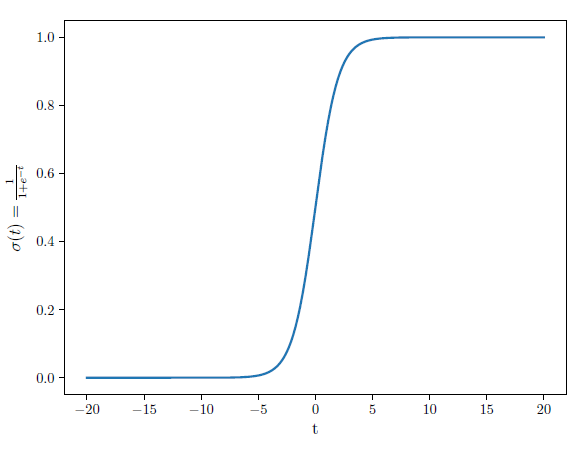
\includegraphics[width=0.8\textwidth]{sigma.png}
  \caption{Sigmoidna funkcija}
  \label{fig:sigmagraph}
\end{figure}

Transformacijom vrednosti linearnog modela, definisana je i zavisnost parametra Bernulijeve raspodele $\mu$ od vrednosti atributa \textit{x}. Slično modelu linearne regresije, forma modela logističke regresije je jednačina: $$  p_w (y=1|x) = \sigma(w \cdot x) $$Izlaz modela je linearna kombinacija njegovog ulaza i koeficijenata. Koeficijenti se dobijaju iz podataka prilikom samog treniranja modela i oni predstavljaju reprezentaciju modela u memoriji \cite{mladen, mlm-logistic-regression}.

Treniranje modela linearne regresije odgovara oceni njegovih parametara i zasniva se na \textbf{principu maksimalne verodostojnosti}. Kao što smo videli, da bi se precizirao statistički model potrebno je uključiti neke parametre. Da bi dobijeni rezultat imao smisla, izbor vrednosti parametara je jako bitan. Jedan od principa izbora ovih vrednosti, princip maksimalne verodostojnosti, je neprihvatanje onih vrednosti parametara za koje su posmatrani podaci malo verovatni. Na taj način biće prihvaćene one vrednosti parametara za koje su posmatrani podaci visoko verovatni \cite{mladen}.

%% RF
\section{Slučajne šume}

\textit{Grupni metodi (eng. Ensemble methods)} su tehnike koje za cilj imaju poboljšanje tačnosti klasifikacije koje se postiže kombinovanjem predviđanja većeg broja klasifikatora. Ovi metodi konstruišu veći broj \textit{baznih klasifikatora} (eng.\textit{ base classifiers}) i kombinovanjem njihovih rezultata vrše svoje predviđanje. Rezultat predviđanja je srednja vrednost u slučaju regresije ili najzastupljenija vrednost u slučaju klasifikacije. Rezultati dobijeni na ovaj način su bolji od rezultata dobijenih korišćenjem samo jednog klasifikatora. \\
Da bi grupni klasifikatori zaista davali bolje rezultate od pojedinačnih klasifikatora, potrebno je da budu ispunjena dva uslova \cite{mitic}:
\begin{enumerate}[1)]
\item bazni klasifikatori treba da budu međusobno nezavisni. U tom slučaju konačna predikcija će biti pogrešna samo ako više od polovine baznih klasifikatora pogreši u predikciji. Potpuna nezavisnost klasifikatora je teško ostvariva, ali se u praksi pokazalo da nije neophodna da bi se ostvarili bolji rezultati. 
\item bazni klasifikatori treba da budu bolji od slučajnog klasifikatora
\end{enumerate}

Osnovna ideja grupnih metoda je kreiranje velikog broja klasifikatora na osnovu trening podataka i neki vid agregacije njihovih rezultata u slučaju nepoznate instance. Grupa klasifikatora može se konstruisati na neki od sledećih načina \cite{mitic}:
\begin{enumerate}[1)]
\item \underline{\textit{Manipulacijom trening podataka}} Ponovnim izborom, u skladu sa izabranom raspodelom, iz originalnog skupa trening podataka kreira se veći broj novih skupova podataka. Raspodela utiče na verovatnoću da će podatak biti izabran za novi trening skup. Zatim se za svaki novi trening skup kreira model klasifikacije izabranim algoritmom (npr. stablo odlučivanja). Dva grupna metoda koja rade na ovaj način su upakivanje i podsticanje.
\begin{itemize}
\item \textit{Upakivanje} (eng. \textit{bagging}) je tehnika koja iznova vrši izbor uzoraka sa zamenom na osnovu uniformne raspodele verovatnoća. Kako sve instance imaju jednaku verovatnoću da budu izabrane, ova tehnika je manje podložna greškama usled preprilagođavanja. Dobijeni skup uzoraka je iste veličine kao i originalni skup. Kako se izbor uzoraka vrši sa zamenom neki podaci će biti izabrani više puta a neki nijednom. Na dobijenim skupovima se treniraju klasifikatori. Nakon što se kreiraju svi klasifikatori moguće je klasifikovati nepoznate instance. Novoj instanci će biti pridružena najzastupljenija klasa.
\item \textit{Podsticanje} (eng. \textit{boosting}) je iterativna procedura koja postepeno menja raspodelu trening podataka i na taj način favorizuje one podatke koji su teži za klasifikaciju. Svakoj trening instanci je pridružen koeficijent težine koji se može promeniti po završetku iteracije. Težine se mogu koristiti bilo kao raspodela pri kreiranju novih skupova podataka bilo za treniranje pristrasnih modela.
\end{itemize}
\item \underline{\textit{Manipulacijom ulaznih atributa}} Novi skupovi trening podataka nastaju kao podskupovi originalnih podataka, slučajnim izborom podataka početnog skupa ili analizom domena. Ovaj pristup daje dobre rezultate u slučaju redundantnih atributa. Slučajne šume su primer metoda koji manipuliše ulaznim atributima i koristi klasifikatore zasnovane na stablima odlučivanja u svojoj osnovi. 
\item \underline{\textit{Manipulacijom algoritma učenja}} Moguće je menjati i sam algoritam učenja. Ovaj način nalazi praktičnu primenu ubacivanjem faktora slučajnosti prilikom treniranja skupa stabala odlučivanja. Umesto izbora najboljeg atributa za podelu u čvoru, moguće je slučajnim izborom odabrati jedan od nekoliko najboljih atibuta podele.
\item \underline{\textit{Manipulacijom oznaka klasa}} Ako je broj klasa dovoljno, veliki višeklasni problem je moguće transformisati u binarni problem podelom oznaka klasa, na slučajan način, u dva disjunktna skupa $A_0$ i $A_1$. Trening podacima čije klase pripadaju skupu $A_0$ pridružuje se klasa 0, a podacima čije klase pripadaju skupu $A_1$ klasa 1. Podaci sa novim oznakama klasa se koriste za treniranje baznog klasifikatora. Grupa klasifikatora se dobija višestrukim ponavljanjem kreiranja skupova $A_0$ i $A_1$ i treniranja klasifikatora nad dobijenim skupovima. Dodeljivanje klase nepoznatoj instanci vrši se tako što svaki bazni klasifikator $C_i$ vrši predviđanje. Ako je predviđena klasa 0, sve klase skupa $A_0$ dobijaju glas. Analogno, ako je predviđena klasa 1, sve klase skupa $A_1$ dobijaju glas. Glasovi se prebrojavaju i rezultujuća klasa će biti ona sa najviše glasova. \par
\end{enumerate}


% naci ovo u miticevoj knjizi
%Slučajne šume nalaze praktičnu primenu zbog otpornosti na greške usled preprilagođavanja koje su karakteristične za stabla odlučivanja. \textit{Stabla odlučivanja (eng. Decision trees)} su popularan metod za rešavanje brojnih problema mašinskog učenja. Često se koriste zbog svoje skalabilnosti, interpretabilnosti i robusnosti pri korišćenju nebitnih atributa. Međutim, stabla odlučivanja su retko tačna. Stabla razvijena previše u dubinu često imaju grešku nastalu preprilagođavanjem. Iako nisu pristrasna, imaju visoku varijansu. Slučajne šume nastaju sa ciljem smanjenja varijanse. Posledica ovoga su nešto veća pristrasnost modela i gubitak interpretabilnosti, ali i znatno poboljšanje performansi izračunavanja. [mitic, wiki-random-forrest]

%Stabla odlučivanja su jednostavna tehnika mašinskog učenja koja ima široku primenu zbog brojnih prednosti. Ovi modeli su jednostavni i jeftini za implementaciju, lako se interpretiraju, robusni su na uticaj šuma, prisustvo redundantnih podataka ne utiče na tačnost modela. Sa druge strane, stabla razvijena previše u dubinu često imaju grešku nastalu preprilagođavanjem

\textit{Slučajne šume} (eng. \textit{Random forests}) pripadaju klasi grupnih metoda. Kao bazni klasifikatori se koriste stabla odlučivanja koja se konstruišu nad skupom nezavisnih slučajnih vektora koji nastaju metodom manipulacije trening podataka. \textit{Upakivanje sa korišćenjem stabala odlučivanja} (eng. \textit{Bagging using decision trees}) je specijalan slučaj slučajnih šuma u kom se slučajnost dodaje u proces pravljenja modela (do sada je postojala u trening podacima) tako što se novi skupovi podataka kreiraju metodom slučajnog izbora sa zamenom od elemenata polaznog skupa. Dodavanje slučajnosti smanjuje korelaciju između stabala, a samim tim i grešku generalizacije cele grupe. Upakivanje popravlja grešku generalizacije smanjujuću varijansu baznih klasifikatora. Pored toga, upakivanje je manje podložno i greškama usled preprilagođavanja, koje je velika mana stabala odlučivanja, zato što nijedna trening instanca nema prednost prilikom izbora, već sve imaju podjednaku verovatnoću da će biti izabrane \cite{mitic}.

%Greška pri generalizaciji teži da raste sa porastom korelacije između stabala. Korelacija među stablima nastaje kada je jedan atribut jak prediktor izlaza. U tom slučaju atribut će se naći u velikom broju stabala, a posledica toga je korelacija među njima.
Svako stablo odlučivanja za podelu u čvoru koristi odgovarajući slučajni vektor podataka koji se dobija na jedan od sledećih načina \cite{mitic}:
\begin{enumerate}[1)]
\item Slučajnim izborom se određuje $F$ atributa koji će se koristiti za podelu u svakom od čvorova (umesto da se za podelu razmatraju svi atributi) nakon čega se stablo konstruiše do kraja bez odsecanja. Ako postoji potreba za većim faktorom slučajnosti moguće je koristiti upakivanje za kreiranje trening skupova. Izbor broja atributa $F$ utiče na snagu i korelaciju modela slučajnih šuma. Za male vrednosti $F$ stabla šume su slabo korelisana, dok veliko $F$ omogućava jače modele zbog korišćenja većeg broja atributa. Često se kao ravnoteža bira $F=log_2d+1$, gde je $d$ broj ulaznih atributa. Ovaj pristup vodi manjem vremenu izvršavanja algoritma jer se prililkom podele u čvoru ne razmatraju svi atributi. 
\item Ako početnih atributa $d$ ima malo, teško je pronaći nezavisni skup slučajnih atributa koji se koriste pri izgradnji modela. Ovo se može prevazići proširenjem skupa atributa njihovom linearnom kombinacijom. Na nivou svakog čvora novi atribut nastaje tako što se metodom slučajnog izbora izabere $L$ atributa iz polaznog skupa, nakon čega se ti atributi linearno kombinuju sa koeficijentima dobijenim iz uniformne raspodele na intervalu [-1,1]. Svaki čvor će dobiti $F$ novih atributa, a najbolji od njih će biti korišćen za podelu čvora. 
\item Mogući pristup podeli unutar čvora je da se umesto najboljeg atributa podele na slučajan način izabere jedan od $F$ najboljih atributa. Stabla dobijena na ovaj način mogu imati veći stepen korelacije u slučaju nedovoljno velikog parametra $F$. Pored toga, ovaj pristup ne daje uštedu u vremenu izvršavanja kao prethodna dva pristupa jer je potrebno ispitati svaki atribut podele u svakom čvoru stabla. 
\end{enumerate}

\section{Mašinsko učenje u Python-u}
,,Python je interpretirani, objektno-orijentisani viši programski jezik sa dinamičkom semantikom. Pythonova jednostavna sintaksa se lako uči i naglašava čitljivost koda koja za posledicu ima nisku cenu održavanja.'' Python podržava veliki broj paketa i modula što vodi ponovnoj upotrebljivosti i modularnosti koda. Nepostojanje faze kompilacije ubrzava čitav proces pisanja i testiranja koda. Debagovanje je prilično jednostavno, greške proizvode izuzetke i ako se oni ne uhvate interpreter ispisuje \textit{stanje steka} (eng. \textit{stack trace}). Štaviše, često je najjednostavniji način debagovanja ubacivanje print naredbi \cite{python-blurb}. %https://www.python.org/doc/essays/blurb/

Autor Pythona je Holanđanin Gido Van Rosum (hol. Guido Van Rossum). %Vremenom njegova uloga kao glavnog razvijaoca Pythona se ne umanjuje, o čemu svedoči titula koju mu je dodelila Python zajednica - Doživotni dobroćudni diktator (eng. Benevolent Dictator For Life). 
Ideju o Pythonu Gido dobija krajem 1980-ih kada je radio kao programer na Državnom institutu za matematiku i informatiku CWI (Centrum voor Wiskunde en Informatica) u jeziku ABC kojim je inspirisan. Implementaciju započinje decembra 1989-te, a prva verzija jezika (verzija 0.9.0) puštena je 1991-ve. Dalji razvoj Pythona se nastavlja. Januara 1994-te izlazi verzija 1.0, unapređena verzija 2.0 izlazi u oktobru 2000-te, a verzija 3.0 u decembru 2008-me \cite{python-history, python-dates}.
%https://www.python-course.eu/python3_history_and_philosophy.php
%https://python-history.blogspot.com/2009/01/brief-timeline-of-python.html   datumi verzija

%Značajno je pomenuti i verzije 2.7.x koje su i dalje u upotrebi. Iako je planirano da se proglase zastarelim 2015-te kada bi se u potpunosti prešlo na verziju 3.0, to je odloženo na 2020-tu zbog velikih razlika između verzija. Pretpostavka je da gomila koda neće raditi na novoj verziji tako da se trenutno uveliko radi na olakšavanju prelaska na novu verziju pomoću programa 2to3. 
%https://legacy.python.org/dev/peps/pep-0373/  2to3

%Jedna od ideja vodilja prilikom razvoja Pythona bila je čitljivost programskog koda i ona je omogućena nazubljivanjem pomoću praznina. Python podržava veliki broj programskih paradigmi uključujući objektno-orijentisanu, funkcionalnu, imperativnu i proceduralnu i takođe ima obimnu standardnu biblioteku. [] %https://en.wikipedia.org/wiki/Python_(programming_language)

\subsection{SciPy ekosistem}
 
\textbf{SciPy} je ekosistem slobodnog softvera za matematiku, nauku i inženjerstvo. Njegovu osnovu čini programski jezik Python i grupa paketa od kojih su za mašinsko učenje najznačajniji \cite{scipy}:
\begin{enumerate}[1)]
\item \textbf{NumPy} je osnovni paket za naučna izračunavanja u Pythonu. Ovaj paket definiše numeričke nizove, matrične tipove, kao i osnovne operacije nad njima.  %https://www.scipy.org/about.html]
%https://docs.scipy.org/doc/numpy/user/quickstart.html
Glavni objekat paketa je homogeni višedimenzioni niz koji je predstavljen kao tabela elemenata (najčešće brojeva), pri čemu su svi istog tipa i indeksirani torkom pozitivnih celih brojeva. Dimenzije niza se nazivaju \textit{osama} (eng. \textit{axis}). Klasa nizova NumPy paketa se naziva \textit{ndarray}.
\begin{itemize}
\item Tačka prostora npr. [1, 2, 1] sa svoje tri koordinate ima jednu osu (dimenziju). Osa se sastoji od 3 elementa pa se kaže da je dužine 3. 
\item Dvodimenzioni niz, npr.
$$[[ 1., 0., 0.],$$ 
$$ [ 0., 1., 2.]] $$
 ima dve ose. Prva osa ima 2 elementa, a druga 3 \cite{scipy-about, scipy-quickstart}. 
\end{itemize}
\item \textbf{Pandas}  %https://pandas.pydata.org/pandas-docs/stable/
je paket koji obezbeđuje strukture podataka za jednostavan i intuitivan rad sa podacima. Predstavlja nadgradnju NumPy biblioteke i napravljen je tako da se lako integriše u razna okruženja koja se koriste za naučna izračunavanja. Pogodan je za podatke koji su smešteni u tabelama, uređene i neuređene vremenske serije, proizvoljne matrice i sve oblike podataka dobijenih na osnovu statističkih posmatranja. Pandas uvodi dve strukture podataka, Series za jednodimenzione podatke i DataFrame za dvodimenzione \cite{pandas}. 
\item \textbf{Matplotlib}  %https://matplotlib.org/ 
je biblioteka koja služi za kreiranje različitih vrsta dijagrama. Većinu dijagrama moguće je kreirati u svega nekoliko linija koda, a sami dijagrami se mogu prilagoditi potrebama korisnika izborom stilova linija (pune, isprekidane,...), svojstava fontova, svojstava koordinatnih osa, itd \cite{matplotlib}.
\end{enumerate}

\textbf{Scikit-learn}  %http://scikit-learn.org/stable/index.html
je modul koji implementira veliki broj algoritama mašinskog učenja. Pored algoritama za rešavanje problema klasifikacije, regresije i klasterovanja ovaj modul podržava i razne tehnike preprocesiranja podataka, kao i tehnike ocenjivanja modela. Zasniva se na bibliotekama NumPy, SciPy i matplotlib \cite{scikit-learn}.



\chapter{Verifikacija softvera}



%\chapter{Primeri korišćenja klasičnih \LaTeX{} elemenata}

% Primeri citiranja
%Ovo je rečenica u kojoj se javlja citat \cite{PetrovicMikic2015}.
%Još jedan citat \cite{GuSh:243}.

% Primeri navodnika
%Isprobavamo navodnike: "Rekao je da mu se javimo sutra".

% Primer referisanja na tabelu (koja se javlja kasnije)
%U tabeli \ref{tbl:rezultati} koja sledi prikazani su rezultati eksperimenta.

% Primer kraćeg ćiriličkog teksta
%{\cir Ово је пример ћириличког текста који се јавља у латиничком документу.}
%U ovoj rečenici se javlja jedna reč na {\cir ћирилици}.

% Primer korišćenja fusnota
%Iza ove rečenice sledi fusnota.\footnote{Ovo je fusnota.}

% Primer dužeg ćirličkog teksta
%\begin{cirilica}
%  Ово је мало дужи блок текста исписан ћириличким писмом у оквиру
%  латиничког документа. Фијуче ветар у шибљу, леди пасаже и куће иза
%  њих и гунђа у оџацима.
%\end{cirilica}

% Primer korišćenja tabele
%\begin{table}
%\centering
%\caption{Rezultati}
%\label{tbl:rezultati}
%\begin{tabular}{c>{\centering}p{2cm}c}
%\toprule
%1 & 2 & 3\\\midrule
%4 & 5 & 6\\\cmidrule(rl){1-2}
%7 & 8 & 8\\
%\bottomrule
%\end{tabular}
%\end{table}

% Primer korišćenja slike
%\begin{figure}[!ht]
%  \centering
%  \label{fig:grafikon}
%  \includegraphics[width=0.5\textwidth]{graph.png}
%  \caption{Grafikon}
%\end{figure}


% Primer jednostavnije matematičke formule
%Evo i jedan primer matematičke formule: $e^{i\pi} + 1 = 0$. 

% Primer referisanja na sliku
%Na slici \ref{fig:grafikon} prikazan je jedan grafikon.

% primer kompleksnije matematičke formule
%$$
%\int_a^b f(x)\ \mathrm{d}x \ =_{def}\ \lim_{\max{\Delta x_k \rightarrow 0}} \sum_{k=1}^n f(x_k^*)\Delta x_k
%$$

% primer referisanja na poglavlja i strane poglavlja
%Više detalja biće dato u glavi \ref{chp:razrada} na strani \pageref{chp:razrada}.

% primer liste
%Možemo praviti i nabrajanja:
%\begin{enumerate}
%\item Analiza 1
%\item Linearna algebra
%\item Analitička geometrija
%\item Osnovi programiranja
%\end{enumerate}

%\pangrami

% ------------------------------------------------------------------------------





% ------------------------------------------------------------------------------

%\pangrami

%\pangrami

% ------------------------------------------------------------------------------
\chapter{Zaključak}
% ------------------------------------------------------------------------------
%\pangrami

%\pangrami

% ------------------------------------------------------------------------------
% Literatura
% ------------------------------------------------------------------------------
\literatura

% ==============================================================================
% Završni deo teze i prilozi
\backmatter
% ==============================================================================

% ------------------------------------------------------------------------------
% Biografija kandidata
\begin{biografija}
%  \textbf{Vuk Stefanović Karadžić} (\emph{Tršić,
 %   26. oktobar/6. novembar 1787. — Beč, 7. februar 1864.}) bio je
%  srpski filolog, reformator srpskog jezika, sakupljač narodnih
%  umotvorina i pisac prvog rečnika srpskog jezika.  Vuk je
%  najznačajnija ličnost srpske književnosti prve polovine XIX
%  veka. Stekao je i nekoliko počasnih mastera.  Učestvovao je u
  %Prvom srpskom ustanku kao pisar i činovnik u Negotinskoj krajini, a
%  nakon sloma ustanka preselio se u Beč, 1813. godine. Tu je upoznao
%  Jerneja Kopitara, cenzora slovenskih knjiga, na čiji je podsticaj
%  krenuo u prikupljanje srpskih narodnih pesama, reformu ćirilice i
%  borbu za uvođenje narodnog jezika u srpsku književnost. Vukovim
%  reformama u srpski jezik je uveden fonetski pravopis, a srpski jezik
  %je potisnuo slavenosrpski jezik koji je u to vreme bio jezik
%  obrazovanih ljudi. Tako se kao najvažnije godine Vukove reforme
%  ističu 1818., 1836., 1839., 1847. i 1852.
\end{biografija}
% ------------------------------------------------------------------------------


\end{document}